% begin module tangent-line-polynomial-power-rule
\begin{frame}
\begin{example}[Calculating the Tangent Line Using the Power Rule]
Find an equation for the tangent line to the parabola $y = \sqrt[3]{x}$ at the point $P = (1,1)$.

\begin{columns}[c]
\column{.4\textwidth}
\uncover<2->{%
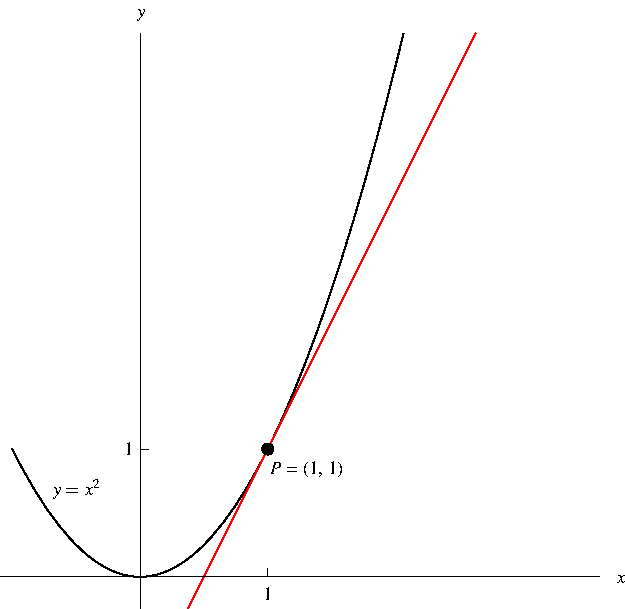
\includegraphics[height=4.5cm]{derivatives/pictures/02-01-secanta.pdf}%
}%
\column{.6\textwidth}
\uncover<2->{%
Here $a = 1$ and $f(x) = \sqrt[3]{x}=x^{\frac{1}{3}}$.
}%
\abovedisplayskip=0pt
\belowdisplayskip=0pt
\abovedisplayshortskip=0pt
\belowdisplayshortskip=0pt

\begin{align*}
\uncover<3->{f'(x)} & \uncover<3->{ = } %
\uncover<3->{\frac{1}{3}x^{\frac{1}{3} - 1} }\\
&\uncover<4->{=} %
\uncover<4->{ \frac{1}{3}x^{\frac{-2}{3} } } \\
&\uncover<5->{ =  } %
\uncover<5->{ \frac{1}{3\sqrt[3]{x^2}}}\\
\uncover<6->{f'(1)} & \uncover<6->{ =  } %
\uncover<6->{\frac{1}{3} } \\
\end{align*}
\uncover<7->{
Point-slope form: $y - 1 = \frac{1}{3}(x - 1)$, or $y = \frac{1}{3}x  +\frac{2}{3}$.
}
\end{columns}
\end{example}
\end{frame}
% end module tangent-line-polynomial-power-rule
